\documentclass[12pt]{article}
    \title{\textbf{Formális nyelvek \\ és automaták}}
    \author{Kidolgozott gyakorlati példák \\ (Szerkesztés alatt álló példatár)}
    \date{}
\usepackage[a4paper,
            left=0.5in,
            right=0.5in,
            top=0.5in,
            bottom=0.5in,
            footskip=.25in]{geometry}
\usepackage{graphicx}
\begin{document}

\maketitle

\section{Mely nyelveket generálják az alábbi grammatikák? \\ Adjuk meg a grammatikák típusait is!}


\subsection{Feladat: \\
$ G=< \{0,1\}, \{S,A,B\}, S, \{ S \rightarrow 01S|1A,\ A \rightarrow B0,\ B \rightarrow 1 \}> $}
\maketitle
\subsection{Megoldás}
A $ S \rightarrow 01S $ szabállyal a '01' stringek számát tudjuk növelni. Majd ha ezt meguntuk, 
az $ S \rightarrow (01)^n1A \vdash (01)^n1B0 \vdash (01)^n110 $ levezetés az egyetlen amivel folytatni tudjuk 
a generálást. Lezárni a generálást csak az $ B \rightarrow 0 $ szabály alkalmazásával tudjuk. \\\\
Tehát a keresett nyelv a következő:
$$ L = \{ \ (01)^n110, \ ahol \ n \in \mathbf{N}  \ \} $$
A G(L) pedig 2-es típusú, azaz környezetfüggetlen, mivel alakja: \\
$ A \rightarrow \omega \ , ahol \ \omega \in (V \cup W)^* , \ valamint \ A \in W^*. $

\subsection{Feladat: \\
$ G=< \{0,1\}, \{S,A,B\}, S, \{ S \rightarrow 0A,\ A \rightarrow 0A|1A|0B|1B,\ B \rightarrow 1B0|10 \}> $}
\maketitle
\subsection{Megoldás}
Kezdetben az $ S \rightarrow 0A $\ szabályt tudjuk csak alkalmazni, ezután viszont választhatunk A és B
generálási irány közül. 
Először válasszuk A irányt: $ 0A \vdash 00A| 01A \ ... $ használatával az első '0' string után
'0'-at vagy '1'-eseket generálhatunk tetszőleges sorrendben és mennyiségben, ez formalizálva így néz ki:
$ 0 \{0,1\}^* $. Ezek után a B irány maradt, ami először egyetlen darab '0'-t vagy '1'-et ad az eddigi string-hez.
A $ B \rightarrow 1B0 $ szabály a bal oldalon az '1'-esek, jobb oldalon a '0'-ák számát tudja növelni
azonos mértékben. Viszont zárásképp '10'-val zárhatunk, ami jó, hiszen ez nem borítja fel az imént leírt
szabályszerűséget. Így most tovább írhatjuk az eddig feltárt $ 0 \{0,1\}^* $ összefüggést:
$ 0 \{0,1\}^*1^m 0^m $. Ámde mert A-ból B-be el kell jutnunk valahogy amit csak egy '0' vagy '1' automatikus
hozzáadásával tehetünk meg, így a képlet $ \{0,1\}^* $ részénél ki kell vennünk az üres szót:
$ \{0,1\}^* \setminus \epsilon $. \\\\ 
Így a keresett nyelv végül a következőképp alakul:
$$ 0 \alpha 1^m 0^m \ | \ \alpha \in \{0,1\}^*\setminus\epsilon \ , \ m \in \mathbf{N}, \ m\geq 1 $$
A G(L) 2-es típusú grammatika. Indoklás a rész legelső feladatánál.


\section{Készítsünk reguláris grammatikákat az alábbi nyelvekhez!}
\subsection{Feladat: \\
$ L=\{ \alpha \in \{ 0,1 \}^* \ | \ \alpha-ra \ igaz \ X \} $ \\
Ahol X az, hogy: nem kezdődik egyessel vagy nem végződik nullára.}
\maketitle
\subsection{Megoldás}
Először is nézzük végig a lehetséges eseteket: 0x0; 0x1; 1x0; 1x1
(itt az x bármilyen és bármennyi véges V*-beli string-et jelöl).
A 'vagy'-al öszekötött állítások igazságértéke csak akkor hamisak ha mindkét állítás hamis.
Ebből az adódik, hogy 0x1 kivételével az összes eset megengedett. \\\\
A grammatika tehát így néz ki: \\
$$ G=<\{ \{0,1\}, \{S,A,B \}, S, \{ S \rightarrow 0|1|1A|0B, \ A \rightarrow 0|1|0A|1A, \ B 
\rightarrow 0B|1B|1 \} \}> $$
A működésének magyarázata esetszétválasztással egyszerűen elintézhető. A kezdőszimbólumból való távozások
közül az B jelöli, hogy egyessel csak végezhetünk ($ B \rightarrow 1 $), 
A pedig hogy bármivel ($ A \rightarrow 0|1 $).
Az $ A \rightarrow 0A|1A $ pedig azt biztosítja, hogyha a kezdő -és zárószimbólum közt bármilyen 
string lehessen, ugyanígy a $ B \rightarrow 0B|1B $
esetnél is.

\subsection{Feladat: \\
$ L=\{ \alpha \in \{ a,b \}^* \ | \ \alpha-ra \ igaz \ X \} $ \\
Ahol X az, hogy: első és utolsó betűje különbözik.}
\maketitle
\subsection{Megoldás}
Először is nézzük végig a lehetséges eseteket: axa; axb; bxa; bxb. Ebből rögtön ki tudjuk szűrni mi kell nekünk:
axb és bxa (itt az x bármilyen és bármennyi véges V*-beli string-et jelöl).
Ezek alapján az előző feladat mintájára tudjuk megkonstruálni a grammatikánkat:
$$ G=<\{ \{a,b\}, \{S,A,B \}, S,
\{ S \rightarrow aB|bA|\epsilon, \ B \rightarrow aB|bB|b, \ A \rightarrow aA|bA|a. \} \}> $$
A működésének magyarázata igen egyszerű és hasonló az előző feladatéhoz:
esetszétválasztást használunk itt is. A B irány it a a-val való kezdést és b-vel való zárást takarja.
Az A irány pedig a fordítottját, azaz a b-vel való kezdést és a-val történő lezárást.
Az $ A \rightarrow aA|bA $ pedig azt biztosítja, hogyha a kezdő -és zárószimbólum közt bármilyen 
string lehessen, ugyanígy a $ B \rightarrow aB|bB $ esetnél is.

\section{Készítsünk (bármilyen) grammatikákat az alábbi nyelvekhez!}
\subsection{Feladat: \\
$ L=\{ a^{2n}b^{3n}ab, \ n \in \mathbf{N} \} $}
\maketitle
\subsection{Megoldás}
Ezt a feladatot sajnos nem tudjuk reguláris grammatikával megoldani, amit készíteni fogunk az \\
környezetfüggetlen lesz. Az ötletünk a következő: $ S \rightarrow aaAbbbab, \ A \rightarrow aaAbbb|aabbb $.
Ezzel először S-ből átmegyünk A-ba, ami azért van mert nem szeretnénk a szó végi 'ab' generálását a szó
belsejében ismételgetni. A-ból viszont véges sokszor tudjuk a szó belsejében az 'aabbb'-k generálását
ismételgetni a $ A \rightarrow aaAbbb $ szabály alkalmazásával. Ha mindezt meguntuk, akkor
a $ A \rightarrow aabbb $ szabállyal zárunk. De ne feledkezzünk meg arról sem, hogy az 'aabbbab' és 'ab'
szavakat is tudnia kell generálnia a grammatikánknak, ezt a $ S \rightarrow aabbbab|ab $ szabályok biztosítják.
Így végül a következő grammatika lesz a megoldás:
$$ G=<\{ \{a,b \}, \{S,A \}, S, \{ S \rightarrow aaAbbbab|aabbbab|ab, \ A \rightarrow aaAbbb|aabbb \} \}> $$

\subsection{Feladat: \\
$ L=\{ 10^{3k}1^{2k}0, \ k \in \mathbf{N} \} $}
\maketitle
\subsection{Megoldás}
A megoldásnál itt is hasonlóan járunk el, mint az előző esetben, szintén környezetfüggetlen grammatikát gyártunk.
Az ötletünk a következő: $ S \rightarrow 000A11, \ A \rightarrow 000A11|00011 $.
Ezzel először S-ből átmegyünk A-ba, ami azért van mert nem szeretnénk a szó eleji '1' és szóvégi '0' 
generálását a szó belsejében ismételgetni. A-ból viszont véges sokszor tudjuk a szó belsejében az '00011'-k
generálását ismételgetni a $ A \rightarrow 00A11 $ szabály alkalmazásával. Ha mindezt meguntuk, akkor
a $ A \rightarrow 00011 $ szabállyal zárunk. De ne feledkezzünk meg arról sem, hogy az '1000110' és '10'
szavakat is tudnia kell generálnia a grammatikánknak, ezt a $ S \rightarrow 1000110|10 $ szabályok biztosítják.
Így végül a következő grammatika lesz a megoldás:
$$ G=<\{ \{0,1 \}, \{S,A \}, S, \{ S \rightarrow 1000A110|1000110|10, \ A \rightarrow 000A11|00011 \} \}> $$

\section{Formális nyelvek metszete, tükörképe és iteráltja}
\subsection{Feladat: \\
$ Legyen \ L_{1}=\{ ab^{n} \ : \ n \in \mathbf{N} \}, \ L_{2}=\{ a^{n}b \ : \ n \in \mathbf{N} \} .$ \\
a) $ L_{1} \cup L_{2} = ?, \ valamint\ L_{1} \cap L_{2} = ? $ \\
b) $ Az \ L_{1}^{*} = \{\alpha^{-1} \ : \ \alpha \in L_{2} \} \ jelolessel, \ L_{1}*L_{2}^{-1}=? $ \\
c) $ Igaz-e, \ hogy \ L_{1}^{*}=L_{2}^{*} \ ? \ Ha\ nem,\ miert?\ Ha\ igen\,\ mi\ ez\ a\ nyelv? $}
\maketitle
\subsection{Megoldás}
Az a) feladatrészre a megoldás a következő: $ L = \{ ab^{n}a^{m}b, \ n,m \in \mathbf{N} \}$, 
mivel a formális nyelvek metszete nem más
mint az összeszorzásuk, ez utóbbi pedig konkatenálást (egymás után illesztést) jelent. \\
A metszet az $ L=\{ ab \} $ lesz, mivel az az az egy szó, ami mindkét nyelvben előfordul. \\\\
A b) feladatrészre a válaszunk: $ L = \{ ab^{n}ba^{m} \ n,m \in \mathbf{N} \} $.
Mivel itt az $ \alpha^{-1} $-en nem jelent mást, mint a $ \alpha $ szó tükörképét, ami valójában az őt alkotó
string-ek fordított sorrendben való egymás utáni leírását takarja. \\\\
Végezetül a c) feladarészhez érkeztünk. Az $ L^{*} = \bigcup_{n \geq 0} L^{n} $ összefüggés jelentését
kell itt tulajdonképp tárgyalnunk. Tehát L nyelv iteráltja nem más, mint a szavainak tetszőleges véges sok
tényezőből álló szorzatainak halmaza. Visszakanyarodva a kérdésünkhöz: az egyenlőség nem teljesül. \\
Indoklás: mivel $ L_{1}=\{ a, ab, abb, abbb, ... \} $ és $ L_{2}=\{ b, ab, aab, aaab, ... \} $ nyelvek szavainak
szorzata között $L_{2}$ esetén előállhat pl. 'bab', de az $L_{1}$ nyelvnél ez nem lehetséges, tehát találtunk
egy ellenpéldát.

\section{Két nyelv metszete és uniója}
\subsection{Feladat: \\
Készítsünk két grammatikát, aminek az uniója az alábbi \\ nyelvet generálja:
$ L=\{ ba^{n}ab^{m}ba \ : \ n,m \in \mathbf{N} \} $}
\maketitle
\subsection{Megoldás}
A nyelvet két részre szedjük és mindkét "részéhez" készítünk egy reguláris grammatikát, majd vesszük a két
grammatika unióját. Megjegyezzük, hogy két grammatika uniója is reguláris kell legyen.
A felosztás nézzen ki a következőképp: $ L_{1}=\{ ba^{n}a \ ...\} $ és $ L_{2}=\{ b^{n}ba \ ...\} $.
Itt fontos megemlíteni, hogy az n hatvány az nyelvenként van érvényben. Tehát az únióban majd végül n és m
fog szerepelni.
Az $ G(L_{1})=\{ ..., \ S \rightarrow bA, A \rightarrow aA|a \} $ generálja, a
$ G(L_{2})=\{ ..., \ S \rightarrow bS|bA, A \rightarrow a \} $ generálja. Ennek a kettőnek a működése
triviális, azokat most terjedelmi okok miatt nem részletezzük. Végül vesszük a két nyelv unióját, ami
valójában a szorzatukat (azaz magyarán egymás után helyezésüket, konkatenálásukat) jelenti.
Ezt úgy érjük el, hogy először a két nyelv terminális jeleinek halmazait diszjunktá tesszük, ez valójában
a "nagybetűk bevesszőzése".
Majd az $L_{1}$ nyelvben a zárószimbólumok végét kiegészítjük a $L_{2}$ grammatika
kezdőszimbólumával, az egyik nyelvből a másikba való átmenet végett. \\\\
Itt megemlítjük azt, hogy ebben a feladatban az $\epsilon$ sehol sem szerepelt a kezdőszimbólumokból kiindulva,
így most ezzel nem kell vacakolnunk. De egyébként ha lenne ilyen arra is kitérünk: \\
Tegyük fel, hogy az $ L_{1} $-ben az $S \rightarrow bA$ helyett az $S \rightarrow bA|\epsilon$ 
szabály szerepel, ekkor $\epsilon$-t csak egyszerűen kivesszük az unióból és helyére az "átvivőszabályt" 
írjuk be, ami jelen esetben az $A \rightarrow aS^{'}$. Ez biztosítja, hogy "semmi" generálás után rögtön a
második nyelv elejére jutunk. Ha az $L_{1}$ és $L_{2}$ nyelvben egyszerre szerepel az $\epsilon$,
akkor egyszerűen az új kezdőszimbólum jobb oldalára be kell írni az $\epsilon$-t is.
Ezek után viszont figyeljünk rá, hogy az új kezdőszimbólum nem fordul elő-e a szabályok jobb oldalán. \\\\
Visszatérve az eredeti feladatunkhoz a megoldás a következőképp alakul: \\
$$ G=<\{ \{a,b\}, \{S,S^{'},A,A^{'},Q \}, Q, \{ Q \rightarrow bA, \ A \rightarrow aA|aS^{'}, \ S^{'} 
\rightarrow bS^{'}|bA^{'}, \ A^{'} \rightarrow a \} \}> . $$

\subsection{Feladat: \\
Készítsünk két grammatikát, aminek a metszete az alábbi \\ nyelvet generálja:
$ L=\{ \alpha ab^{n}b \ |\ \alpha \in \{ \epsilon, a, b \} \ , \ n \in \mathbf{N} \} $}
\maketitle
\subsection{Megoldás}
A nyelvet két részre szedjük és mindkét "részéhez" készítünk egy reguláris grammatikát, majd vesszük a két
nyelv metszetét, ami az összeadásukat jelenti. Az összeadás itt valami olyasmit takar, hogy egyik vagy
másik nyelv generálható, hozzátéve hogy mindkét nyelv nem generálható egyszerre, de legalább az egyik
mindeképp generálható. \\
Az $L_{1}=\{ ..., \ aab^{n}b \}$ legyen, az $L_{2}=\{ ..., \ bab^{n}b \}$. Ezek után az $L_{1}$ és $L_{2}$-höz
késztünk grammatikákat, úgy hogy a kezdő szabályokhoz még egy $\epsilon$-t is beveszünk. \\
A követkőképpen néznek ki:
$G(L_{1})=\{ ..., \ S \rightarrow aA|\epsilon,\ A \rightarrow aB,\ B \rightarrow bB|b \}$, valamint
$G(L_{2})=\{ ..., \ S^{'} \rightarrow bA^{'}|\epsilon,\ A^{'} \rightarrow aB^{'},\ B^{'} \rightarrow bB^{'}|b \}$.
Már a terminális jelek diszjunktá tétele is megtörtént.
Ezek után nincs más dolgunk, minthogy bevezetünk egy új kezdőállapotot, amiből elérhetővé tesszük az
$L_{1}$ és $L_{2}$ béli szavakat is. Tehát $G(L)=\{..., \ Q \rightarrow aA|bA^{'}|\epsilon \}$, majd ezek után
az összes szabályt változatlanul bemásoljuk:
$G(L)=\{..., \ Q \rightarrow aA|bA^{'}|\epsilon, A \rightarrow aB, B \rightarrow bB|b, A^{'} \rightarrow aB^{'},
B^{'} \rightarrow bB^{'}|b \}$. Mivel $Q \rightarrow \epsilon$ szerepel, így át kell néznük, hogy Q nem-e fordul
elő a szabályok jobb oldalán, de nem. Jók vagyunk! A teljes megoldás így írható fel:
$$ G(L)=<\{ \{ a,b \}, \{ S,S^{'},A,A^{'},B,B^{'},Q \}, \ Q, \{ Q \rightarrow aA|bA^{'}|\epsilon, A \rightarrow 
aB, B \rightarrow bB|b, A^{'} \rightarrow aB^{'}, B^{'} \rightarrow bB^{'}|b \}\}> $$

\subsection{Feladat: \\
Készítsünk reguláris grammatikát, ami az alábbi nyelvet generálja:
$ L=\{ 00, 111 \}^* $ ahol a terminális jelek halmaza: $ \{0, 1\} $}
\maketitle
\subsection{Megoldás}
Intuitíve felírjuk a megoldást, majd indokoljuk annak helyességét:
$$ G(L)=<\{ \{ 0,1 \}, \{ S,A,B,C,D,E \}, \ S, $$ $$ \{ S \rightarrow \epsilon|0A|1C, A \rightarrow 
0B, B \rightarrow 1C|0A, C \rightarrow 1D, D \rightarrow 1E|1C, E \rightarrow 0A \}\}> $$
Az indoklás a következőképp néz ki: \\ Az ABC-ben szerepelhet az üres szó is, 
így rögtön az $S \rightarrow \epsilon$ szabállyal kezdünk, viszont ekkor a szabályok jobb oldalán S már nem
szerepelhet, erre kell figyelnünk. Aztán az $ S \rightarrow 0A|1C$ szabályok közül az egyik alkalmazásával
eldöntjük, hogy a '00'-kat vagy az '111'-eseket szeretnénk először generálni. A $B \rightarrow 0A$-val folytatjuk a
'00'-ák generálását, a $B \rightarrow 1C$-vel pedig áttérünk az '111'-ek generálására. Ugyanezt amit eddig 
csinűltunk a '0'-k generálásával, most eljátszuk az '1'-kel is, tehát: $D \rightarrow 1C$-vel újra egyeseket 
generálgatunk, míg $D \rightarrow 1E$ és $E \rightarrow 0A$ szabályok használatával át tudunk térni a '0'-k 
képzésére is. Összefoglalva: a $B \rightarrow 1C|0A$ és $D \rightarrow 1E|1C$ állapotok a konstrukció központi 
működtető elemei, itt tudunk váltani a '00'-ák és '111'-ek generálása közt, az $E \rightarrow 0A$ szabályt 
pedig abból kifolyólag kellett bevezetnünk, hogy az S nem szerepelhet a jobb oldalon az üres szó miatt.

\section{A formális nyelvek mint halmazok}
\subsection{Feladatok és megoldásai: \\}
$ V=\{ a,b,c \}, \ W=\{ c,d,e \} .$ \\\\
$ V*(W \setminus V)*W^* \ =\ \{a,b,c\}*\{d,e\}*\{\epsilon, c, d, e, cd, ec, ed, cde, ecd, ...\} $ \\
$= \{ad, ae, bd, be, cd, ce\}*\{\epsilon, c, d, e, cd, ec, ed, cde, ecd, ...\} = \{ ad\alpha,
ae\alpha, bd\alpha, be\alpha, cd\alpha, ce\alpha \} $, ahol $\alpha \in \{c,d,e \}^{*}$ \\\\
$ (V \setminus W)(W \setminus V) \ =\ \{a,b\}*\{d,e\} = \{ ad, ae, bd, be \} $ \\
$ V^* \setminus W^*\ \Longrightarrow \ $ Minden lehet vélgülis, csak az $\epsilon$-okat
és a 'c'-t vettük ki. Tehát minden $\{ a,b,c,d,e \} $-t tartalmazó szó kijöhet, ami nem tartalmaz
$\epsilon$-t és nem csak 'c'-ből áll (c lehet benne).



\section{Véges determinisztikus automaták készítése a megadott nyelvhekhez}
Először is megjegyezzük, hogy a V minden 7-es ponthoz tartozó feladatnál $V=\{0,1\}$.
\subsection{Feladat:}
$ L_1 = \{ \alpha \in V^* : \alpha $ pontosan három darab 1-esre végződik $\}$
\begin{figure}[h]
  \centering
  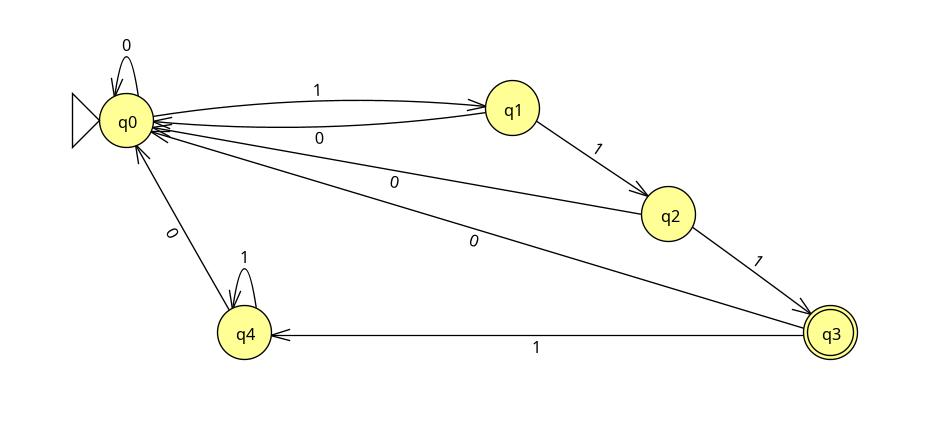
\includegraphics[width=0.7\linewidth]{img/a.jpg} 
  \caption{fnya.pdf/141.oldal/4.23. a) feladatrész}
  \label{fig:your_label}
\end{figure}
\subsection{Megoldás:}
A képen látható az elkészített automata, indoklása a következő: \\
A $q_0 \rightarrow q_1 \rightarrow q_2 \rightarrow q_3$ állapotok közt csak '1'-esek szerepelnek mindenütt, ez
azért van mivel $\alpha$ szónak pontosan 3db '1'-re kell végződnie. De a szó kezdődhet '0'-val is, így $q_0$
állapotba vezethet önmagába '0'-ás nyíl. Továbbá a kezdőállapotból indulva és '1'-est olvasva mindig
visszaugorhatunk a keződállapotba, ahol csupa nullákat ismerhetűnk fel, ez a "visszaugráló" és "önmagába nullát
vezető" konstrukció együttesen biztosítja, hogy az automata a 3db '1'-es előtt még bármit fel tudjon ismerni.
A $q_3$-ból $q_4$-be mutató '1'-es nyílra azért van szükségünk mert a szóban valahol, bárhol előfordulhat 4 vagy 
több egymás utáni '1'-es és ezeket is fel kell tudnunk ismerni.
\subsection{Feladat:}
$ L_2 = \{ \alpha \in V^* : \alpha $ -ban a 010 előfordul részszóként $\}$
\begin{figure}[h]
  \centering
  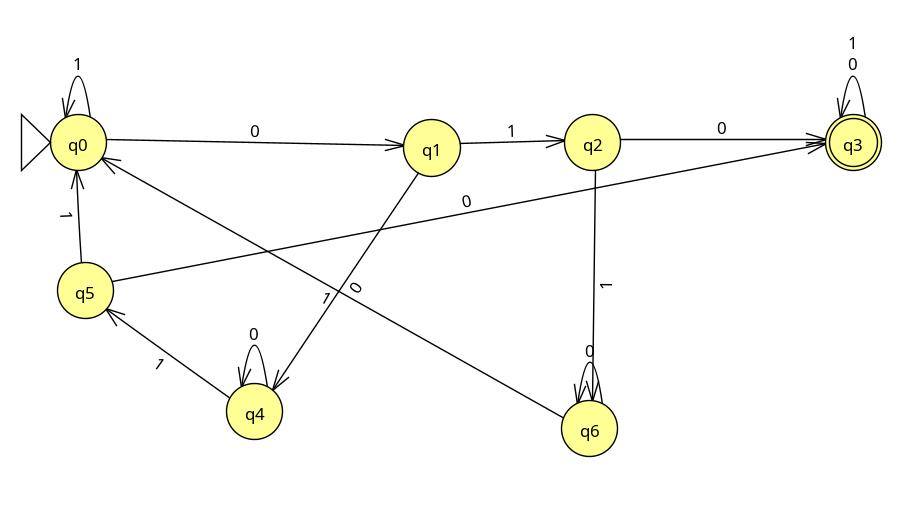
\includegraphics[width=0.7\linewidth]{img/b.jpg} 
  \caption{fnya.pdf/141.oldal/4.23. b) feladatrész}
  \label{fig:your_label}
\end{figure}
\subsection{Megoldás:}
A képen látható az elkészített automata, indoklása a következő: \\
A $q_0 \rightarrow q_1 \rightarrow q_2 \rightarrow q_3$ állapotokon megintcsak kötelező végigfutnunk, ezek
biztosítják, hogy a legrövidebb szót, a '010'-át az automata felismerje. A logika egyébként hasonlít az előző 
példához: itt is az "önmagába (most) 1-et vezető" + "visszaugráló" stratégiát alkalmazzuk. Magyarán értjük, hogy
a keződállapotban az önmagába mutató nyíl miért kell, a végállapotban azért, mivel a '010' sztring után még
bármit olvashatunk. A visszaugrálást most is az a probléma szülte, hogy a szó nem csak '0'-val, hanem bármivel 
kezdődhet: a $q_2$-ből $q_6$-ba fordulás ezzel magyarázahtó, a $q_1$-ből való lefordulás utáni 
$q_4 \rightarrow q_5$ közti '1'-es esetén egyszerre kell figyelembe venni, hogy $q_5$-ből mehetünk a 
végállapotba is, tehát '010'-át kell képznünk, és azt is, hogy a kezdőállapotba csak '1'-essel mehetünk vissza,
hogy az erdeti konstrukciónkat ne rontsuk el.
\subsection{Feladat:}
$ L_3 = \{ \alpha \in V^+ : \alpha $ nem kezdődik két egymás utáni 0-val $\}$
\begin{figure}[h]
  \centering
  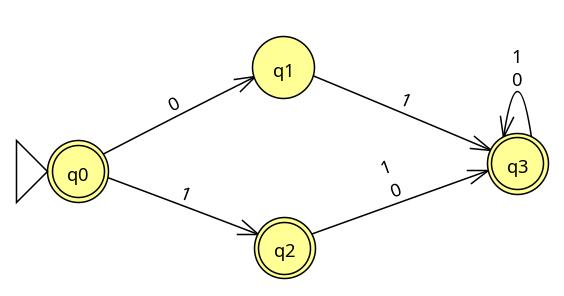
\includegraphics[width=0.7\linewidth]{img/c.jpg} 
  \caption{fnya.pdf/141.oldal/4.23. c) feladatrész}
  \label{fig:your_label}
\end{figure}
\subsection{Megoldás:}
A képen látható az elkészített automata, indoklása a következő: \\
A $q_0$ keződállapotból '0' hatására és '1' hatására két különböző irányba indulunk el, szétválasztva ezzel
azt az esetet amikor kötelezően '1'-nek kell jönnie, ill. amikor '0' vagy '1' is jöhet. A végállapotokból az 
olvasást folytathatjuk amíg tetszik, mivel a szó végére nincs kikötés a feladatban.
\subsection{Feladat:}
$ L_4 = \{ \alpha \in V^* : \alpha $ az 101 valamilyen pozitív kitevős hatványával kezdődik $\}$
\begin{figure}[h]
  \centering
  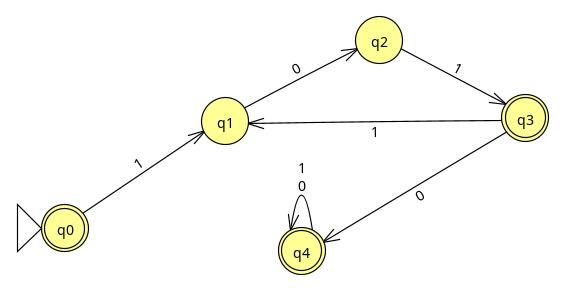
\includegraphics[width=0.7\linewidth]{img/d.jpg} 
  \caption{fnya.pdf/141.oldal/4.23. d) feladatrész}
  \label{fig:your_label}
\end{figure}
\\ Megjegyzés: a feladatot úgy értelmezzük, hogy az n-ik beolvasott '101' után csak '0'-val tudunk kilépni
a ciklusból, és folytatni az olvasást.
\subsection{Megoldás:}
A képen látható az elkészített automata, indoklása a következő: \\
A $q_0$ kezdőállapot egyben végállapot is lehet, ez azért van mivel '101' nulladik hatványa $\epsilon$ lesz.
Az automata kötelező jelleggel beolvassa a '101' sztinget mindimum 0 szor ill. 1-szer, aztán ha ezt ismételgetni
szeretnénk, akkor a $q_3$ végállapotból '1'-est olvasva megtehetjük még tetszőlegesen sokszor. Amint ezt meguntuk,
mindenképp legalább egy '0'-át kell olvasnunk, hogy a '101' szó "lezáruljon". Így aztán $q_4$-ben, a szó végén
meg bármit tudunk olvasni, mivel a szó végére nincs kikötés.
\subsection{Feladat:}
$ L_5 = \{ \alpha \in V^* : \alpha $ -ban van pontosan k darab egymás utáni 1-es $\}$
\begin{figure}[h]
  \centering
  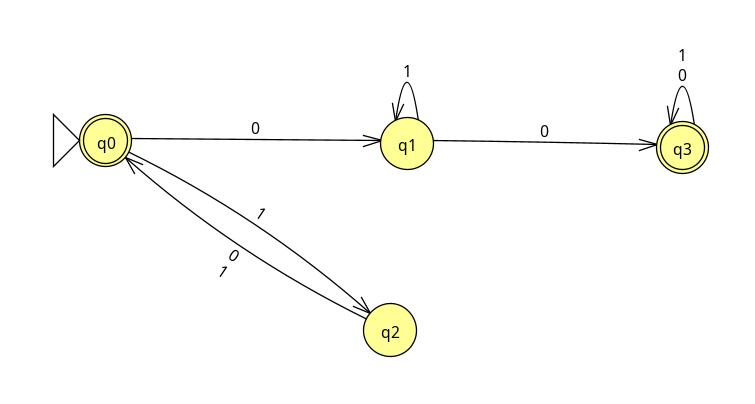
\includegraphics[width=0.7\linewidth]{img/e.jpg} 
  \caption{fnya.pdf/141.oldal/4.23. e) feladatrész}
  \label{fig:your_label}
\end{figure}
\subsection{Megoldás:}
A képen látható az elkészített automata, indoklása a következő: \\
A 'k' darab egymás utáni '1'-es lehet a szó közepén, végén, elején, bárhol... az iménti első kettő esetet a 
$q_1$ ill. $q_3$ önmagába mutató nyilukkal oldottuk meg. Amint a szó elején fordul elő k darab egymás utáni
'1'-es, úgy akkor a $q_2$ állapotba való megfordulás lesz a megoldás.

\section{Véges nemdeterminisztikus automaták készítése a megadott nyelvhekhez}
\subsection{Feladat:}
$ L=\{ \alpha \in \{0,1\}^* : \alpha $ első betűje egy '1'-es és van benne valahol pontosan 
3db egymást követő '1'-es $ \} $
\begin{figure}[h]
  \centering
  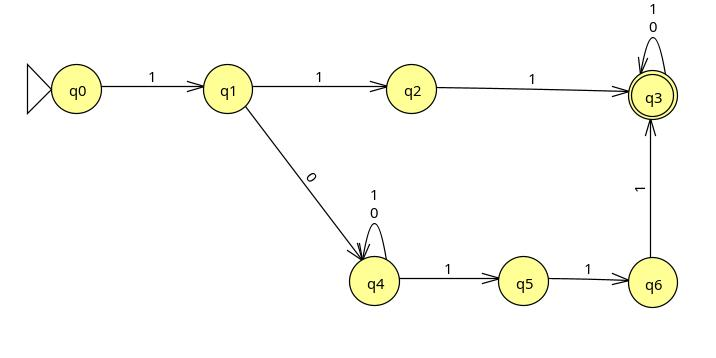
\includegraphics[width=0.7\linewidth]{img/nd_01.jpg} 
  \caption{előző évi zárthelyi dolgozatokból}
  \label{fig:your_label}
\end{figure}
\subsection{Megoldás:}
A képen látható az elkészített automata, indoklása a következő: \\
A $q_0 \rightarrow q_1 \rightarrow q_2 \rightarrow q_3$ átmenet nemcsak azt biztosítja, hogy a szó '1'-essel
kezdődjön, hanem azt is hogy a legrövidebb szót (a 3db '1'-est) felismerje, amikor ezt megtette, akkor bármit
olvashat (ez a $q_3$ önmagába mutató nyilainak magyarázata). Ámde néznünk kell azokat az eseteket is, amikor
a szó ugyan 1-essel kezdődik, de utána '0' van, és a '111' sztring pedig valamikor máskor fordul elő a szóban.
Ezeket az eseteket hivatott reprezentálni a $q_1 \rightarrow q_4$ átmenet, és az azt követő állapotok.
\subsection{Feladat:}
$ L=\{ \alpha \in \{a,b\}^* : \alpha $ utolsó betűje (pontosan) egy 'b' és van benne valahol pontosan 
4db egymást követő 'b' $ \} $
\begin{figure}[h]
  \centering
  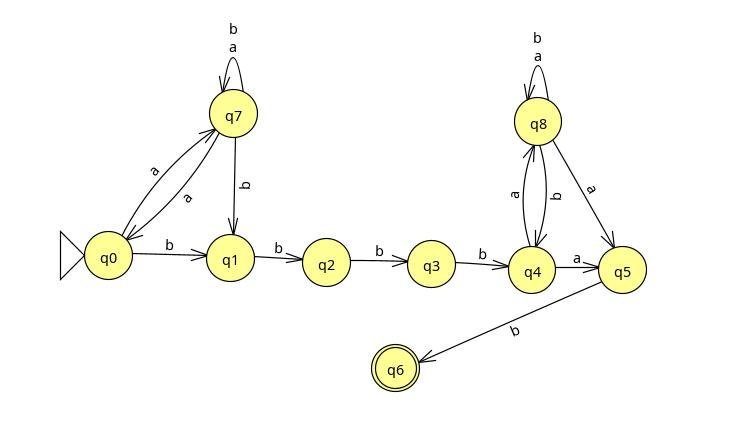
\includegraphics[width=0.7\linewidth]{img/nd_ab.jpg} 
  \caption{előző évi zárthelyi dolgozatokból}
  \label{fig:your_label}
\end{figure}
\subsection{Megoldás:}
A képen látható az elkészített automata, indoklása a következő: \\
A $q_0 \rightarrow q_1 \rightarrow q_2 \rightarrow q_3 \rightarrow q_4 \rightarrow q_5 \rightarrow q_6$ 
átmenetekkel biztosítjuk a legrövidebb szó felismerését, ez a 'bbbbab'.
Mivel a 4db 'b' bárhol előfordulhat a szóban, ezért a 'bbbb' sztring első 'b'-je előtt vagy épp az utolsó 'b'-je
után le kell ágaznunk 'a' sztringet olvasva ($q_0$ és $q_4$). Az itteni "leágazásokkal" lehetővé tesszük bármilyen
karakter olvasását bármennyiszer, ám kikötjük hogy a végén úgy is 'b'-t ill. 'a'-t kell olvasnia, hogy a 
'bbbb'+utolsó egy 'b' sztring felismerésére épített konstrukció ne romoljon el.

\section{A kis Bar-Hillel lemma és alkalmazása}
\subsection{Lemma:}
Legyen adva egy L nyelv, amelyet egy determinisztikus véges automata felismer. Ekkor van olyan n természetes
szám, hogy ha az $\alpha$ szó az L nyelvnek olyan eleme, amelyre $|\alpha| \geq n$, akkor $\alpha$ előállítható
$\alpha=uvw$ alakban, ahol $|uv| \leq n, |v| \geq 1$, és minden i = 0,1,2,... természetes számra az $uv^iw$ szavak
szintén benne lesznek a nyelvben. Erre a továbbiakban csak Bar-Hillel lemma néven hivatkozunk.
\subsection{Megjegyzés:}
A gyakorlat során a fenti lemmát arra tudjuk használni, hogy ellenpélda kereséssel bebizonyítsuk egy nyelvről,
hogy az nem ismertethető fel véges determinisztikus automatával, vagy továbbgondolva: a nyelv maga nem reguláris.
\subsection{Alkalmazása:}
1.) Igazoljuk, hogy az $L=\{ \alpha\alpha^{-1}:\alpha\in\{a,b\}^* \}$ nyelv nem reguláris. \\\\
Megfelelő ellenpélda:\\
Legyen $\alpha\alpha^{-1}=$ a...ab$|$ba...a, tehát $\alpha=a...ab$ és $\alpha^{-1}=ba...a$, eddig jók vagyunk.\\
Ez a szó azért tökéletes, mert kielégíti a Bar-Hillel lemma feltételeit:\\
$\alpha = n('a')+1('b') = n+1,$ így $\alpha \geq n$,\\
valamint: $|uv| \leq n$ és a $|v| \geq 1$, ami azért igaz, mert a fölbontást az alábbiak szerint csináltuk:\\
$\alpha=$ 1 darab 'a' (=:u) + min.1 darab 'a' (=:v) + 1 darab 'b' (=:w)\\
Ámde ha az így kapott $\alpha$ szóban a v-k számát iteráljuk, akkor az $\alpha\alpha^{-1}$ szó már nem lesz
szimmetrikus. Magyarán a fölbontásunk kielégíti a lemma feltételeit, viszont a lemma azt mondja ki, hogy
az ilyen szavak benne lesznek a nyelvben, mi pedig ezzel ellentmondásra jutottunk, hisz látjuk hogy a
(szimmetria hiánya miatt) nincs benne.
\\\\
2.) Igazoljuk, hogy az $L=\{ \alpha 0\alpha^{-1}:\alpha\in\{0,1\}^* \}$ nyelv nem reguláris. \\\\
Megfelelő ellenpélda:\\
Legyen $\alpha 0\alpha^{-1}=$ 0...01$|$0$|$10...0, tehát $\alpha=0...01$ és $\alpha^{-1}=10...0$, 
eddig jók vagyunk.\\
Ez a szó azért tökéletes, mert kielégíti a Bar-Hillel lemma feltételeit:\\
$\alpha = n('0')+1('1') = n+1,$ így $\alpha \geq n$,\\
valamint: $|uv| \leq n$ és a $|v| \geq 1$, ami azért igaz, mert a fölbontást az alábbiak szerint csináltuk:\\
$\alpha=$ n darab '0' (=:u) + min.1 darab '0' (=:v) + 1 darab '0'+'1' (=:w)\\
Ámde ha az így kapott $\alpha$ szóban a v-k számát iteráljuk, akkor az $\alpha\alpha^{-1}$ szó már nem lesz
szimmetrikus (most az ne tévesszen meg minket, hogy közöttük van egy '0'). 
Magyarán a fölbontásunk kielégíti a lemma feltételeit, viszont a lemma azt mondja ki, hogy
az ilyen szavak benne lesznek a nyelvben, mi pedig ezzel ellentmondásra jutottunk, hisz látjuk hogy a
(szimmetria hiánya miatt) nincs benne.
\\\\
3.) Igazoljuk, hogy az $L=\{ b\alpha b\alpha^{-1}:\alpha\in\{a,b\}^* \}$ nyelv nem reguláris. \\\\
Megfelelő ellenpélda:\\
Legyen $b\alpha b\alpha^{-1}=$ ba...aa$|$baa...a, tehát $\alpha=a...aa$ és $\alpha^{-1}=aa...a$, 
eddig jók vagyunk.\\
Ez a szó azért tökéletes, mert kielégíti a Bar-Hillel lemma feltételeit:\\
$\alpha = 1('b')+n('a') = 1+n,$ így $\alpha \geq n$,\\
valamint: $|uv| \leq n$ és a $|v| \geq 1$, ami azért igaz, mert a fölbontást az alábbiak szerint csináltuk:\\
$\alpha=$ 1 darab 'b' (=:u) + min.1 darab 'a' (=:v) + 1 darab 'a' (=:w)\\
Ámde ha az így kapott $\alpha$ szóban a v-k számát iteráljuk, akkor az $\alpha\alpha^{-1}$ szó már nem lesz
szimmetrikus. Magyarán a fölbontásunk kielégíti a lemma feltételeit, viszont a lemma azt mondja ki, hogy
az ilyen szavak benne lesznek a nyelvben, mi pedig ezzel ellentmondásra jutottunk, hisz látjuk hogy a
(szimmetria hiánya miatt) nincs benne.
\\\\
Megjegyzés: \\
Ezek könnyűnek tűnhetnek, viszont ha egy reguláris nyelvre pl.: 010$\alpha$-ra eljátszuk ugyanezt, észrevesszük,
hogy akármilyen szó akármelyik részét iteráljuk, mindig benne lesz a nyelvben (010-val fog kezdődni).
Természetesen a fenti állítás csak akkor igaz, ha a fölbontás kielégíti a Bar-Hillel lemma feltételeit.\\

\section{Figyelem! A következő (11-14) pontokhoz terjedelmi okok miatt
már csak 1-1 db kidolgozott példa fog tartozni.}

\section{Nemdeterminisztikus automata determinisztikussá tétele}
\subsection{Példa:}
A 8-as ábra bal oldalán adva van egy véges nemdeterminisztikus automata. Hogyan készítünk vele ekvivalens
determinisztikus automatát? Megtehetetnénk azt is, hogy meghatározzuk az automata által felismert nyelvet, majd
ehhez a nyelvhez készítünk egy determinisztikus automatát. De ehhez egyrészt gondolkodnunk kell, másrészt pedig
ez sok esetben nem célravezető, ugyanis nemdeterminisztikus automatát készíteni egy nyelvhez sokkal egyszerűbb,
mint determinisztikusat, ezért van szükségünk erre a a következő algoritmus jellegű dologra:\\\\
A $q_1$ állapotból indulunk, megnézzük hogy az automata 'a' és 'b' jelek hatására merre mennek:\\
$\rho (q_1,a)=\{q_1,q_2\}$, valamint $\rho (q_1,b)=\{q_3\}$. \\ 
Most akkor vizsgáljuk hogy: $\rho (q_2,a)=\{q_3\}$, $\rho (q_2,b)=\{q_1\}$, igen ám...
de mostmár ne feledkezzünk meg arról hogy $\{q_1,q_2\}$ állapothalmazról van szó, tehát az imént kapott
állapotokat össze kell unióznunk a $q_1$ esetén kapottakkal, ez a következőképp néz ki:
$\rho(\{q_1,q_2\},a)=\{q_1,q_2,q_3\}$, $\rho(\{q_1,q_2\},b)=\{q_1,q_3\}$.
Most akkor ugyanezt kell lezongoráznunk $\{q_1,q_3\}$ és $\{q_1,q_2,q_3\}$ állapothalmazokkal:\\
$\rho(\{q_1\},a)=\{q_1,q_2\}$, $\rho(\{q_1\},b)=\{q_3\}$\\
$\rho(\{q_3\},a)=\{q_1\}$, $\rho(\{q_3\},b)=\{q_2,q_3\}$\\ 
Ezek közül a $\{q_2,q_3\}$ állapothalmazok még nem léteznek, tehát ezeket fel kell rajzolnunk.
S aztán ugyanígy meg kell néznünk, hogy a halmaz állapotaiból 'a'-k és 'b'-k hatására merre mennek nyilak.
Az algoritmus akkor áll le, ha azt vesszük észre hogy már nem tudunk új állapotot vagy állapothalmazt felrajzolni.
Jelen esetben ez most történt meg.

\begin{figure}[h]
  \centering
  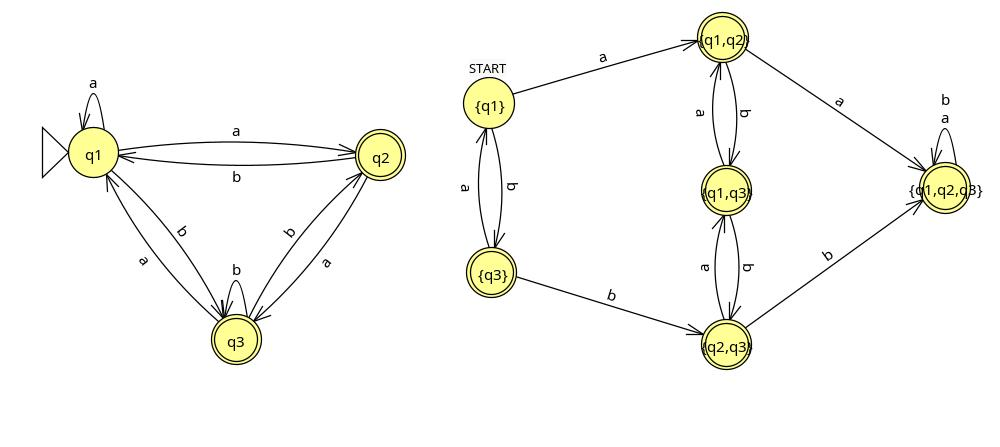
\includegraphics[width=0.7\linewidth]{img/nemdet_to_det.jpg} 
  \caption{N.K.G. algoritmusok}
  \label{fig:your_label}
\end{figure}

\section{Reguláris grammatika $\rightarrow$ automata konverzió}
\subsection{Példa:}
Adott a következő reguláris grammatika. Készítsünk el egy olyan automatát, amely azokat a szavakat ismeri föl
amelyeket a nyelvtan generál.
$$ G=<\{ \{a,b\}, \{S,A,B \}, S,
\{ S \rightarrow aB|bA|\epsilon, \ B \rightarrow aB|bB|b, \ A \rightarrow aA|bA|a. \} \}> $$
A grammatika nemterminális jelei felelnek meg az automata állapotainak, a kezdőszimbólum a kezdőállapotnak.
A jelek (nemterminálisok) mindenhol jelek maradnak...
Ha a grammatika tudja generálni az $\epsilon$-t, akkor az automata kezdőállapotát egyben végállapottá is
tesszük. Amelyik nemterminálisból indulva a nyelvtannal a generálást be tudjuk fejezni, azokat az automata
állapotok esetén bevezetjük egy teljesen új végállapotba.

\begin{figure}[h]
  \centering
  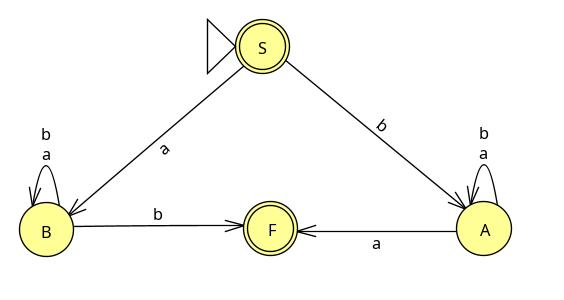
\includegraphics[width=0.7\linewidth]{img/g_to_a.jpg} 
  \caption{N.K.G. algoritmusok}
  \label{fig:your_label}
\end{figure}

\section{Automata $\rightarrow$ reguláris grammatika konverzió}
\subsection{Példa:}
Adott az alábbi véges determinisztikus automata. Készítsünk olyan reguláris grammatikát, amely azokat a szavakat
generálja, amelyeket az automata felismer.
\begin{figure}[h]
  \centering
  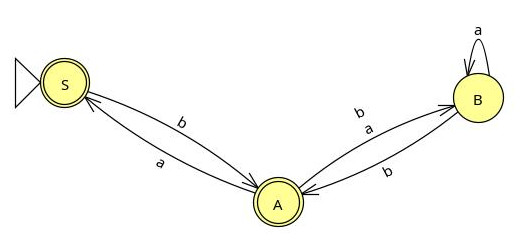
\includegraphics[width=0.7\linewidth]{img/a_to_g.jpg} 
  \caption{N.K.G. algoritmusok}
  \label{fig:your_label}
\end{figure}\\
A megoldás a következőképpen fog kinézni:
$$ G=<\{ \{a,b\}, \{S,A,B,S^{'} \}, S,
\{ S \rightarrow \epsilon|bA|b, \ B \rightarrow aB|bB|aS^{'}, \ A \rightarrow aB|bA, \ S^{'} \rightarrow bA|b \} 
\}> $$
Most az előző feladatot fogjuk visszafelé játszani: az állapotokból lesznek a nemterminális jelek.
\\
Itt arra kell figyelnünk, hogyha a kezdőállapot egyben végállapot is, akkor az automata felismeri az üres szót,
ilyenkor viszont a szabályok jobb oldalán nem állhat a kezdőszimbólum. Ezt úgy tudjuk kiküszöbölni, hogy
a nemterminális jelek közé felveszünk egy újat, amikből elérhetővé tudjuk tenni azokat a szabályokat is, amik
az eredeti kezdőszimbólumból voltak az $\epsilon$ (üres szó) kivételével.

\section{Automata minimalizáló algoritmus}
\subsection{Példa:}
sf jdf\\kjldfgjd\\l fkdjjd\\pokdfoij\\opkgjroig\\odjgi

\end{document}
